\chapter{Introduction \& Motivation}
\label{chapter:introduction}
\begin{music}
    \parindent10mm \instrumentnumber{1} \setstaffs1{1} 
    \generalmeter{\meterfrac34} \generalsignature{3}
    \startextract
            \Notes \Dqbu dk \zhl{i*} \en
        \bar
            \Notes \Dqbu hi \zhu{h*} \en
    \zendextract
\end{music}
\epigraph{\textit{one thing that won't change with time is the memories of younger years}}{Minuet of Forest --- Ocarina of Time}

We are living in the wake of milestones in biotechnology and computational biology that suggest reverse-engineering cell biology is within our grasp. The coronavirus pandemic accelerated investment in biotechnology \cite{DeFrancesco2021Financing2020}. The fields of synthetic and systems biology are beginning to resemble engineering disciplines; genetic engineering is becoming more precise, high-throughput single-cell experiments are performed by robots and measurements across all levels of the central dogma are possible: genomics, transcriptomics, proteomics and metabolomics \cite{Perkel2021Single-cellAge}. Advances in micro-fabrication \cite{Shafiee2017TissueMedicine} and in-vitro reconstitutive methods \cite{Gopfrich2018MasteringCells} have allowed biologists isolate pathways and mechanisms to a level of mathematical and computational tractability \cite{Sharpe2017ComputerTomorrow.}.

The complexity barrier in biology poses a significant challenge. Systems and synthetic biology have historically made progress through a process of brute force trial and error. This usually involves the interaction of many custom-made parts that are iteratively optimised by human intervention. A trend first observed in the 1980s known as \textit{Eroom's law} revealed that discoveries in biotechnology are becoming slower and more expensive over time, despite improvements in technology \cite{Scannell2012DiagnosingEfficiency}. This problem is exemplified by the declining success rate of clinical trials in the drug discovery process \cite{Wong2019EstimationParameters} and compounded by the ongoing reproducibility crisis \cite{Ioannidis2005WhyFalse.,Mullard2021HalfEffort}. It appears that much of the low-hanging fruit has been picked \cite{Earm2014IntegrativeDevelopment} with methodologies whose standards for transparency, reproducibility and accessibility leave us with much to be desired. Despite the widespread lack of mechanistic understanding in human cell biology, sophisticated engineering goals such as targeted modification of the immune system are now possible. In 2018, a chimeric antigen receptor T-cell therapy --- \emph{tisagenlecleucel} \cite{Halford2021TisagenlecleucelConsiderations} --- for the treatment of adolescent and young adult acute lymphoblastic leukaemia became the most expensive cancer therapy ever, at \$475,000. In settings where biomanufacturing relies on specific known mechanisms, but otherwise involve a greater number of unknown mechanisms, a vast amount of omics data is collected along key protocol stages in a attempts to understand and optimise production.

After a decade of engineering advances in data science and machine learning, epitomised by deep learning methods, theoretical foundations on high-dimensional learning tasks are beginning to condense \cite{Bronstein2021GeometricGauges}. Many tasks such as computer vision, playing Go, or protein folding are in fact feasible with appropriate computational scale. Remarkably, the essence of deep learning is built from two simple algorithmic principles: the notion of lower-dimensional \emph{representation}, whereby group equivariant and invariant transformations are composed to capture the appropriate notion of regularity for each task \cite{Bronstein2021GeometricGauges}, and second, learning by local gradient-descent type methods enabled by \emph{differentiable programming} \cite{Innes2019AComputing}.

The emerging picture suggests that bringing together the advances in software and wetware in iterative hypothesis generation and discovery pipelines are key to overcoming the complexity barrier in biology \cite{Sharpe2017ComputerTomorrow.,Ringel2020BreakingLaw,AlQuraishi2021DifferentiableMechanisms}. The term \textit{in silico} has become popularised amongst biologists, which conceptualises a computational model, alongside \emph{in vitro} and \emph{in vivo}, as a method for investigating an organism \emph{in situ}. Researchers are going as far as conceptualising the \emph{digital twin} for personalised medicine \cite{Bjornsson2019DigitalMedicine}. Bringing together deep learning and biomedical research has the potential of importing the notions of \emph{representation} and \emph{differentiability} into experimental protocols \cite{AlQuraishi2021DifferentiableMechanisms} and thereby reaping their benefits. Differentiability within experimental pipelines has the same advantage over brute force trial and error as it does over sampling-based algorithms and thereby decrease the time and cost for biological research. While not all equipment, data and resources used to perform a study can be shared, \emph{representations} of a study in the form of computational models can increase transparency and reproducibility. Efforts towards open standards have gained traction over the past decade \cite{Malik-Sheriff2020BioModels15Science} with model sharing standards such as Systems Biology Markup Language \cite{Hucka2018TheCore} and data repositories like Human Cell Atlas
\cite{Regev2017TheAtlas} and Flow Repository \cite{Spidlen2012PreparingFlowRepository.org}. The open standards and ethical thresholds of deep learning are also increasing, with the formation of OpenAI \cite{Brockman2016OpenAIGym} and sharing standards such as ONNX \cite{Bai2019ONNX:Exchange}.

In this thesis we focus on the benefits of \emph{representation} and \emph{differentiability} in the context of the genetic engineering of cell phenotypes in synthetic biology. In Chapter \ref{chapter:background} we introduce the reader a relevant background in differential equations and machine learning with applications in cell biology to set the stage for the publications in Chapters \ref{chapter:double-exclusive}--\ref{chapter:exploring}. We will see how a differential equation \emph{representation} of a cell or population of cells requires an exploration of the relationship between \emph{bifurcation theory} and the concept of a \emph{phenotype}. Chapter \ref{chapter:double-exclusive} exhibits the results of an interdisciplicary collaboration between in synthetic biology, during which an iterative \emph{design--learn} workflow was followed in an attempt to overcome the biological complexity barrier. During this collaboration, a disconnect between design goals and parameter inference methods was identified which lead to the novel \emph{bifurcation} inference method published in Chapter \ref{chapter:inference}. Chapter \ref{chapter:exploring} is an adaptation of a publication, in preparation at the time of writing this document, that explores the importance of interactive exploration of high-dimensional flow cytometry data for immunophenotyping. Finally, Chapter \ref{chapter:conclusions} concludes with retrospectives on the previous chapters, which includes a revised view of a \emph{design--learn} workflow for synthetic biology, that in principle is completely \emph{differentiable}. Furthermore, we propose how one would use concepts from Chapters \ref{chapter:inference}--\ref{chapter:exploring} to interactivity explore the space of hypotheses that \emph{represent} the same cell phenotype. Our conclusions would be most impactful in cell line development where flow cytometry and other omic-type measurements are taken at different protocol stages of a biomanufacturing process.

\section{Representation of Single Cells}

While we focus on differential equation \emph{representations} of single cells, they are only one of many \emph{representations}. In this section we give a brief motivation behind why differential equations were chosen, what other representations exist and how results may translate between differential equations and other representations. When studying a particular biological phenomenon, the appropriate spatio-temporal scale must be chosen that simplifies the mechanism under study while preserving the relationships between experimentally accessible parameters and the resultant behaviours. Unlike in many physical sciences, we do not expect a single unifying tractable model of biological mechanisms under study. In practice there exist multiple equally valid models with variously degrees of complexity. The paradigm of \emph{top--down} and \emph{bottom--up} modelling methods (Figure \ref{fig:tdbu}) emerged as a means of navigating different scales and complexities.

\begin{Figure}
    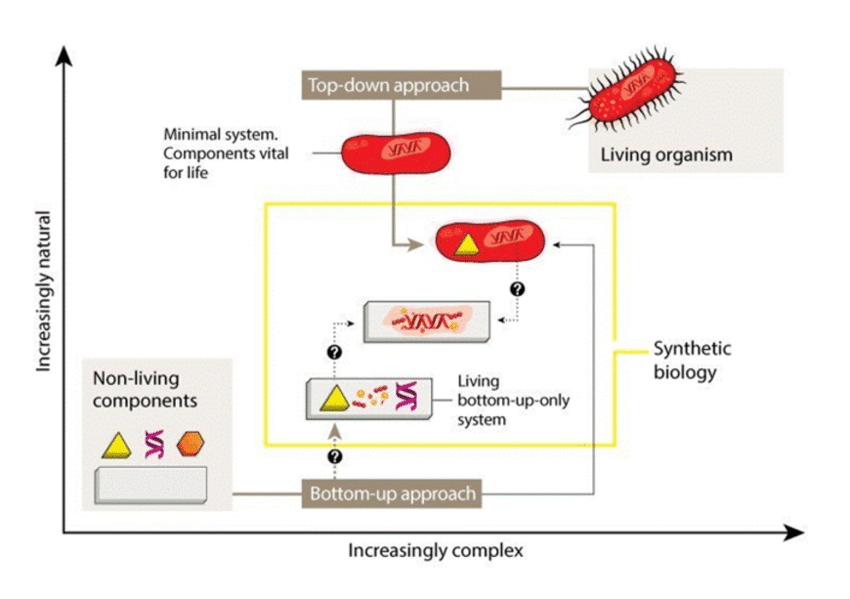
\includegraphics[width=80mm]{figures/top-down-bottom-up.png}
    \caption{Top-down and bottom-up modelling for single cells}
    \label{fig:tdbu}
\end{Figure}

Differential equations are convenient because they are \emph{differentiable}, continuous state and continuous time models and hence are already compatible with the two algorithmic principles of deep learning \cite{Bronstein2021GeometricGauges}. In the context of \emph{dynamical systems theory} it is relatively simple to derive analogous results for discrete state or discrete time models: cellular automata \cite{}, Markov chains \cite{}, stochastic processes \cite{}, discrete maps \cite{} just to name a few. As long as the model is differentiable, we can proceed to use it in optimisation routines. In practice, with automatic differentiating tools at our disposal most programmes become differentiable in most places...This is because while one could use a sigmoidal-type functions as a differentiable substitutes for conditional branching in the control flow of a program, one is still forced to evaluate multiple passes of the program before getting an accurate estimate of the derivative of the program. At best a program can be piecewise differentiable

It is important to choose a time-scale and space-scale that is relevant to the problem. If one is interested in tissue dynamics, attempting to model DNA conformations within each cell will render the problem intractable. As George Booth aptly put \textit{``most models are wrong but some are useful"} so the role of theoretical descriptions in these settings is not necessarily to describe the way reality \textit{is} but serve as tools to bridge the non-intuitive gap between bottom-up and top-down approaches. 

\subsection{Model Reduction}
Sloppiness and sensitivity analysis have been extensively used in the
search for reduced models. Linear mappings between models that preserve stoichiometry and reactant structure were investigated \cite{Cardelli2014MorphismsFunction,Cardelli2017MaximalSystems} and computational tools based on partition-refinement were released \cite{Cardelli2017ERODE:Equations}. Structural similarity between reaction networks can be revealed by such mappings, elucidating the functional aspects of complex networks in terms of simpler networks. The aim of the Design--Learn pipeline is to extend this framework to nonlinear mappings with an emphasis on geometry rather than kinetics. Most inference techniques attempt to match geometry and kinetics simultaneously in an attempt to obtain a quantitative model. This thesis emphasises that geometry alone should be prioritised in order to obtain qualitatively equivalent models. Furthermore recent results in pattern formation theory \cite{Halatek2018} do not depend on kinetics at all, only geometry.

Following the initial literature on smooth and match estimators
\cite{Gugushvili2012Smoothing} -- which overcome the bottleneck
having to integrate a proposed hypothesis for every parameter update --
a plethora of methods for the inference of differential equations
became available \cite{Brunton2016SparseSINDYc,GorbachScalableSystems}.
The essence of these methods is to estimate the derivatives of the
data rather than integrate the model and simultaneously estimate 
the qualitative and quantitative behaviours. In most biological
experiments batch-to-batch variations decrease the certainty
with which it is possible to quantify a behaviour. Whether or not
a parameter is identifiable, reduntant or sloppy have become
key questions in biology \cite{Chis2016OnIdentifiability,
Gabor2017ParameterBiosystems,Villaverde2016StructuralModels}.

\section{Differentiability in Experimental Protocols}

While there is a clear mathematical definition of what a \emph{differentiable program} \cite{Innes2019AComputing} is, what does it mean for experimental protocols in biology to be \emph{differentiable}? In the effort to introduce transparency and reproducibility in experimental methods in synthetic biology, a standard for the Design--Build--Test--Learn cycle has emerged (Figure \ref{fig:dbtl}). This workflow has now been established as a paradigm with some aspects that have been automated by liquid handling robots, bioreactor environments and image processing pipelines. However, humans in the loop and custom moving parts still persist. The challenge in automating these processes lies in defining a programming interface that has a sufficiently high-level of abstraction for transparent implementation while allowing for customisation \cite{Abate2018ExperimentalSemantics}.

\begin{Figure}
    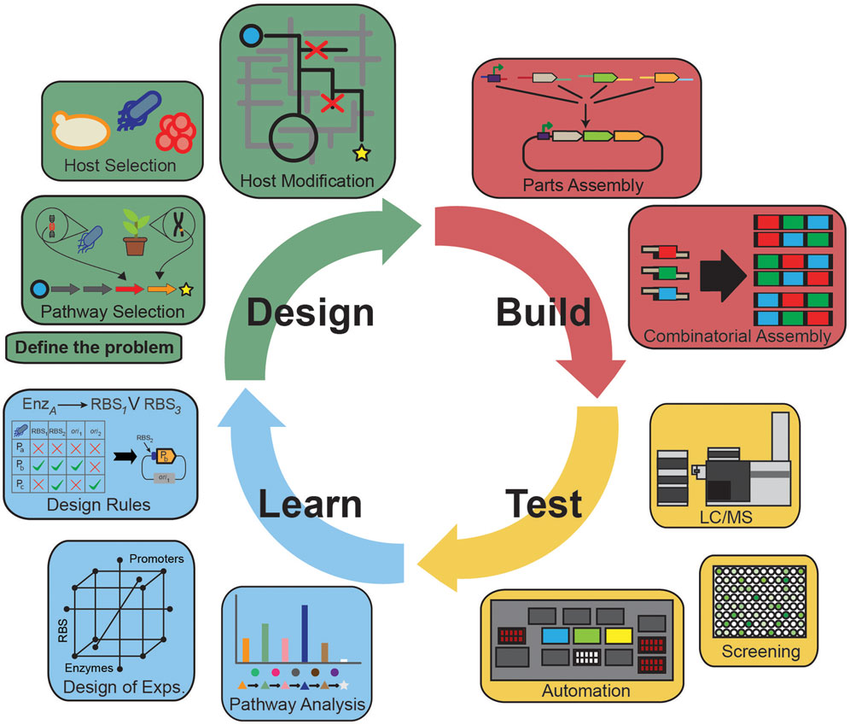
\includegraphics[width=60mm]{figures/dbtl.png}
    \caption{Design-Build-Test-Learn cycle from synthetic biology}
    \label{fig:dbtl}
\end{Figure}

In principle,

This thesis will focus on modelling and inference using systems of differential and partial differential equations, which fits into the Design--Learn part of the cycle. Differential equations occupy a small subset of possible modelling tools, however they are amongst the most popular due to their ease of use formulation and simulation. This ease of access creates a zoo of models in literature making it difficult to identify the key ingredients that distinguish different models. Furthermore the relationship between multiple plausible \textit{and} in-plausible hypotheses is rarely investigated. This motivates desire for an automated Design--Learn pipeline -- outlined in Section \ref{section:design-learn} -- which can generate and catalogue models in a transparent manner while producing insights for the Build stage. This pipeline is applied in an experiment-theory collaboration described in
Chapter \ref{chapter:double-exclusive}.

Fortunately for biologists copies of the target of their reverse-engineering attempts are available all around us. Less fortunate is the fact that most attempts at deconstructing the cell end in loss of function and destruction of the individual components. This restriction motivates system biologists to manipulate environmental signals \textit{in vivo} and build mechanistic models from correlations between signals and responses \cite{Triantafillou2017PredictingCells}. Models focus on relationships between macroscopic variables where the underlying mechanisms are not known.

\subsection{Design--Learn Workflow}
\label{section:design-learn}

This section outlines the proposal for a design--learn pipeline for
the purposes of model reduction and system design. Suppose experimental
collaborators have provided us with time-course gene expression data $\mathcal{D}$,
which could be taken via time-lapse microscopy of cells growing on microfluidic plates,
optical density measurements from microtiter plate assays or temporal snapshots of
flow cytometry measruements. On the other hand one may want to specify a behaviour
$\mathcal{H}$ which may have not yet been observed. This would be specified with
top-down constraints, i.e. there exist oscillations of a fixed frequency or
a region of bistability.

The experimentalists may want to know whether the data collected could
result in a model of predictive power without mechanistic knowledge
of the underlying biochemistry. Moreover it would be desirable gain insights
in parameter regimes in the vicinity of observations, without having to
wait for the theorists to produce a refined model. Such real-time insights
would guide data collection protocols, optimising the amount of information
gained while keeping the number of experiments performed to a minimum. Often
data is noisy and at worst case contradictory; these issues must also be exposed.

\begin{Figure}
    \begin{tikzpicture}[node distance=2cm]

        \node (nonparametric) [process, minimum width=5cm] {non-parametric inference};
        \node (data) [io, right of=nonparametric, xshift=1cm, yshift=2cm] {observations $\mathcal{D}$};

        \node (field) [decision, below of=nonparametric] {field $\Vector{f}$};
        \node (pred) [io, right of=field,  xshift=2cm] {predictions};

        \draw [arrow] (data) |- (nonparametric);
        \draw [arrow] (nonparametric) -- (field);
        
        \draw [arrow] (field) -- (pred);
        \draw [arrow,color=BurntOrange] (pred) -- +(0,3.5);

    \end{tikzpicture}
    \caption{Workflow loop for optimal experimental design, without mechanistic model}
    \label{fig:experimental-design}
\end{Figure}
\noindent
Figure \ref{fig:experimental-design} outlines the workflow for optimal experimental design.
The term \textit{non-parametric} defines the procedures that have prioritised  
functional generality and flexibility over mechanistic insights gained from the values
of the parameters and shapes of the mathematical forms. Neural networks and Gaussian process
regressors are examples of non-parametric estimation procedures, which produce an estimate
of the field $\Vector{f}$ that predicts gene expression rates at given expression levels.
Based on these predictions, the experimentalist may proceed to collect data in the most
informative parameter regions, which would in turn more accurately estimate $\Vector{f}$.

\label{section:refinement}
Often predictions from field $\Vector{f}$ are not enough. Models constructed
with feasible biophysical assumptions $\Vector{h}(\Vector{\theta})$ have the potential
to extrapolate predictions and give concrete biophysical meanings to each parameter $\Vector{\theta}$.
This way the experimentalist knows exactly which modification to the system they must
make in order to achieve a desired behaviour. More often than not it is also unclear
whether the model and its assumptions are reasonable, which brings us to the desire
to score our hypotheses. For increased
accuracy and efficiency \cite{Meeds2019EfficientSystems} the mechanistic model
$\Vector{h}(\Vector{\theta})$ is inferred against non-parametric estimate $\Vector{f}$
rather than the data $\mathcal{D}$ directly. Furthermore as discussed in Section
\ref{section:geometry} the aim is to optimise geometry rather than kinetics.
Alternatively one may construct $\Vector{h}(\Vector{\theta})$ to cover a whole class
of models, such as those that satisfy mass-action. The expectation is that most of the
parameters would be zero but some would be informative. One can obtain a distribution
of optimal parameters $\rho(\Vector{\theta})$ by running multiple optimisations. From
this distribution one may construct alternative hypotheses and update $\Vector{h}(\Vector{\theta})$.
By iterating this procedure one would identify the minimal model within the model class that
explains the data. This process is known as model refinement or reduction.

\begin{Figure}
    \begin{tikzpicture}[node distance=2cm]

        \node (field) [decision] {field $\Vector{f}$};
        \node (hypothesis) [io, left of=field,  xshift=-2cm] {hypothesis $\Vector{h}(\Vector{\theta})$};
        \node (parametric) [process, below of=field, minimum width=5cm] {geometric inference};
        
        \node (params) [io, below of=parametric] {parameter distribution $\rho(\Vector{\theta})$};
        \node (score) [io, right of=params, xshift=4cm] {score};
        \node (decomp) [process, below of=params, minimum width=5cm] {clustering and decomposition};
        \node (models) [io, left of=decomp, xshift=-3cm] {models};

        \draw [arrow] (field) -- (parametric);
        \draw [arrow] (hypothesis) |- (parametric);
        \draw [arrow] (parametric) -- (params);
        
        \draw [arrow] (params) -- (decomp);
        \draw [arrow] (params) -- (score);
        \draw [arrow] (decomp) -- (models);
        \draw [arrow,color=ForestGreen] (models) -- +(0,5.5);

    \end{tikzpicture}
    \caption{Overview of hypothesis scoring pipeline and model refinement loop}
    \label{fig:non-parametric}
\end{Figure}

Suppose now that refined mechanistic models of the form $\Vector{h}(\Vector{\theta})$
have been obtained using the model refinement loop. These could be a library of known
parts that have been individually characterised, but never combined to form a larger
system. The experimentalists would like to create a system with a specified behaviour
$\mathcal{H}$ and would like to know which parts to combine and which modifications
to make. The model refinement loop can be used with the design as an input.

\begin{Figure}
    \begin{tikzpicture}[node distance=2cm]

        \node (nonparametric) [process, minimum width=5cm] {non-parametric inference};
        \node (design) [io, left of=nonparametric, xshift=-1cm, yshift=2cm] {design $\mathcal{H}$};

        \node (field) [decision, below of=nonparametric] {field $\Vector{f}$};
        \node (hypothesis) [io, left of=field,  xshift=-2cm] {models $\Vector{h}(\Vector{\theta})$};
        \node (parametric) [process, below of=field, minimum width=5cm] {geometric inference};
        
        \node (params) [io, below of=parametric] {parameter distribution $\rho(\Vector{\theta})$};

        \draw [arrow] (design) |- (nonparametric);
        \draw [arrow] (nonparametric) -- (field);
        
        \draw [arrow] (field) -- (parametric);
        \draw [arrow] (hypothesis) |- (parametric);
        \draw [arrow] (parametric) -- (params);

    \end{tikzpicture}
    \caption{Overview of system design pipeline}
    \label{fig:design}
\end{Figure}